\documentclass[12pt,a4paper]{article}
\usepackage[utf8]{inputenc}
\usepackage[english]{babel}
\usepackage[margin=2cm]{geometry}
\usepackage{amsmath}
\usepackage{amsfonts}
\usepackage{amssymb}
\usepackage{graphicx}
\usepackage{pgfplots}
\usepackage{url}
\usepackage[square,numbers,sort&compress]{natbib}
%\pgfplotsset{compat=1.13}
\newcommand{\ratelaw}{\theta(\mathbf{s},\mathbf{p})}
\renewcommand*\rmdefault{bch}
\newcommand{\wolf}[1]{{\color{red} [#1]}}
\renewcommand{\thefigure}  {S\arabic{figure}}

\title{Genome-scale architecture of small molecule regulatory networks and the fundamental trade-off between regulation and enzymatic activity - Supplementary Text}

\begin{document}
\maketitle
\tableofcontents
\pagebreak
\section{Futile Cycles and Small Molecule Regulation}
We gathered information regarding reactions that are involved in futile cycling (also known as Type II extreme pathways \cite{Price2002-ef}), using the \emph{E. coli} genome scale model iJO1366 \cite{Orth2011-qi} and the COBRApy toolbox \cite{Ebrahim2013-vw}. First, we converted it to an irreversible model, by splitting each reversible reaction into two distinct irreversible ones and allowing only zero or positive fluxes. We constrained all exchange reactions to have no flux, and added the following ATP generating reaction with a constant positive flux (e.g. $1$):
\begin{equation}
ADP + P_i + H^+ \rightharpoonup ATP + H2O~.
\end{equation}
Then, we solve the mass-balance problem while minimizing the sum of all fluxes, which finds the shortest futile cycle. We then eliminate the cycle by constraining its reaction to have zero flux, and iteratively run the minimization until no more solutions are found. We found 58 non-overlapping futile cycles, majority of which comprising 2 reactions.

We mapped these reactions to enzymes, using EC number information (where available) and ended up with 75 unique reactions that take part in futile cycles (\texttt{FutileCycleReactionsECnumber.csv}). From these, using our SMRN, we find that 37 are regulated by at least one small molecule, whereas 38 are not regulated (\texttt{FutileCycleRegulatoryInfo.csv}).

\begin{center}
\begin{tabular}{|l|c|c|}
	\hline
    & In Futile Cycle & Not in Futile Cycle  \\ \hline
Regulated by small molecule & 37 & 327  \\ \hline
Not regulated & 38 & 266 \\ \hline
\end{tabular}
\end{center}

Using a right-tailed Fischer’s exact test (fishertest function, MATLAB) to detect if there are significantly more small molecule regulation in futile cycle participating reactions, we verify that there is no significant overrepresentation of regulation in reactions that take part in futile cycling (p = 0.86).
The code for this analysis and its results are freely available on our GitHub repository (\url{https://github.com/eladnoor/small-molecule-regulation}).

\section{Reaction Reversibility and Small Molecule Regulation}

We used reactions’ $\Delta_r G'^\circ$ together with reaction stoichiometry and standard physiological metabolite concentrations of substrates or products and calculated a reversibility index (denoted $\Gamma$) quantifying the extent to which each reaction is thermodynamically reversible \cite{Noor2012-mp}:

\begin{eqnarray}
	\ln(\Gamma) &\equiv& \frac{2}{N_s+N_p} \cdot \left( \frac{\Delta_r G'^\circ}{RT} + (N_p - N_s)\cdot \ln (0.001) \right)
\end{eqnarray}
where $N_s$ and $N_p$ are the number of substrates and products respectively (excluding water).
The threshold value we considered for reversibility is $\Gamma$ = 1000, as it represents a relative concentration range of 1000 for all substrates and products. Any reaction with a value of $\Gamma$ higher than 1000 was assumed to be irreversible whereas when $\Gamma < 1000$, it was considered to be reversible. We mapped this information to central carbon metabolism reactions, and ended up with 32 reversible and 8 irreversible reactions. From these, using our SMRN, we found that 19 reversible reactions are known to be regulated by small molecule(s), whereas 13 are not. Regarding irreversible reactions, we found that 7 are known to be regulated, whereas 1 is not known to be regulated by any small molecule. 

\begin{center}
	\begin{tabular}{|l|c|c|}
		\hline
		& Reversible & Irreversible \\
		& $\Gamma \leq 1000$ & $\Gamma > 1000$ \\ \hline
		Regulated by small molecule & 19 & 7  \\ \hline
		Not regulated & 13 & 1 \\ \hline
	\end{tabular}
\end{center}
We consequently performed Gene Set Enrichment Analysis using the Fischer exact test and verified that there is no significant over-representation of regulation in reactions with larger reversibility indexes (p-value: 0.1). Expanding our analysis to the full SMRN network, we again find no statistical significance (p-value = 0.25):
\begin{center}
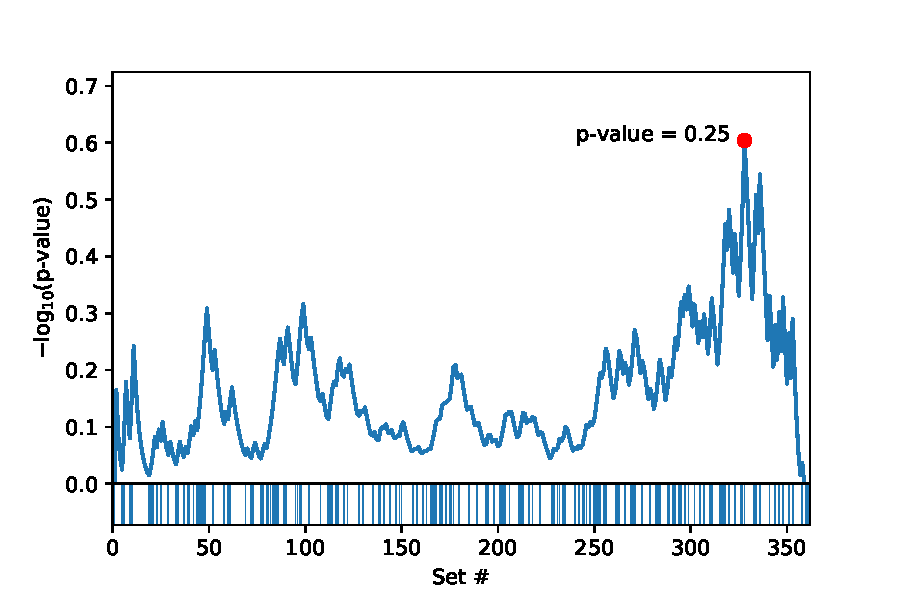
\includegraphics[width=0.7\textwidth]{../manuscript/figS10.pdf}
\end{center}

\section{Metabolic Control Analysis}
\subsection{What is elasticity?}
Metabolic Control Analysis \cite{Fell1996-be} is a mathematical framework to understanding the dynamics and control of metabolic networks. In particular, it defines local properties called elasticities that can be used to quantify how the control of metabolic fluxes depends on other quantities in the system (\textit{i.e.} the topology of the metabolic network, and the levels of metabolites). \emph{Scaled elasticity} is defined as the infinitesimal response of a single flux ($v$) to one of the parameters ($a$), using a partial derivative of the log-scaled functions:
\begin{eqnarray}
    \varepsilon_a^v \equiv \frac{\partial \ln(v)}{\partial \ln(a)} = \frac{\partial v}{\partial a} ~ \frac{a}{v}
\end{eqnarray}

The elasticity has several properties which make it desirable for modeling metabolic systems. In particular, for a variety of kinetic rate laws (\textit{e.g.} Michaelis-Menten kinetics), the elasticity (for Michaelis-Menten kinetics, the substrate elasticity is bounded between 0 and 1). 

\subsection{Single-substrate Control in Michaelis-Menten Kinetics}
To illustrate the concept of elasticity, let us consider an enzyme-catalyzed reaction, described by a one-substrate irreversible Michaelis-Menten kinetic rate law:
\begin{eqnarray}
    v &=& V^+ ~ \frac{s}{K_M + s}
\end{eqnarray}
where $s$ is the substrate concentrations (in units of molar), and $K_M$ is the Michaelis-Menten coefficient (also in molar).

\begin{center}
	\begin{tikzpicture}
	\begin{loglogaxis}[width=200pt,axis x line=bottom, axis y line=left, tick align=outside, domain=1e-2:1e3, xlabel=$s/K_M$, ylabel=$\frac{s}{K_M + s}$]
	\addplot+[mark=none,smooth] (\x,{(\x/(1+\x))});
	\end{loglogaxis}
	\end{tikzpicture}
\end{center}

The scaled elasticity for $s$ is given by:
\begin{eqnarray}
    \varepsilon_s^v &=& \frac{\partial v}{\partial s} ~ \frac{s}{v} = V^+ ~ \frac{K_M + s - s}{(K_M + s)^2} ~ \frac{s}{v} \nonumber \\
    &=& \frac{K_M}{(K_M + s)^2} ~ (K_M + s) = \frac{K_M}{K_M + s} = 1 - \frac{s}{K_M + s}\label{eq:eps_s_v_irr}
\end{eqnarray}

\begin{center}
	\begin{tikzpicture}
	\begin{semilogxaxis}[width=200pt,axis x line=bottom, axis y line=left, tick align=outside, domain=1e-2:1e3, xlabel=$s/K_M$, ylabel=$\varepsilon_s^v$]
	\addplot+[mark=none,smooth] (\x,{(1/(1+\x))});
	\end{semilogxaxis}
	\end{tikzpicture}
\end{center}

Note that the scaled elasticity is bounded between 0 and 1. More specifically, $\varepsilon_s^v$ is maximized (\textit{i.e.} the substrate has the highest control potential) at low substrate concentrations, and minimized at high substrate concentrations.

As shown by \citet{Noor2013-vv}, this formula for substrate elasticity can be generalized to reversible Michaelis-Menten reactions \cite{Hofmeyr1995-fl, Rohwer2010-tx}, where the saturation term is separated from the thermodynamic term:
\begin{eqnarray}\label{eq:rev_mm}
    v &=& V^+ \cdot \kappa \cdot \gamma \nonumber\\
    \kappa &\equiv& \frac{s/K_S}{1 + s/K_S + p/K_P} \nonumber\\
    \gamma &\equiv& 1 - \frac{p/s}{K_{eq}'}
\end{eqnarray}
where $p$ is the product concentration, $K_S$ and $K_P$ are the Michaelis-Menten constants for the substrate and product, and $K_{eq}'$ is the apparent equilibrium constant. In this case, the elasticity of the substrate is:
\begin{eqnarray}
    \varepsilon_s^v &=& \gamma^{-1} - \kappa
\end{eqnarray}

Finally, in order to compare this result to the irreversible case, we show that
\begin{eqnarray}\label{eq:reversible_substrate_eps}
\varepsilon_{s}^v &=& \gamma^{-1} - \kappa = \left(1 - \frac{p/s}{K_{eq}'}\right)^{-1} - \frac{s/K_S}{1 + s/K_S + p/K_P} \nonumber\\
&>& 1 - \frac{s/K_S}{1 + s/K_S + p/K_P} > 1 - \frac{s/K_S}{1 + s/K_S} = 1 - \frac{s}{K_s + s}\,,
\end{eqnarray}
which is exactly the elasticity of the substrate in the irreversible case (Equation \ref{eq:eps_s_v_irr}). So, assuming a reaction is irreversible provides an underestimation of the elasticity. Nevertheless, in cases where $p \rightarrow 0$, we can see that $\varepsilon_{s}^v \rightarrow 1 - \frac{s}{K_s + s}$.

\subsubsection{Reversible Monod-Wyman-Changeux Kinetics}
A common model for cooperativity in enzyme kinetics was developed by Monod-Wyman-Changeux (MWC kinetics). It is described by the same 3-term rate law as reversible Michaelis-Menten kinetics (Equation \ref{eq:rev_mm}), but with a different expression for $\kappa$:
\begin{eqnarray}
\kappa_n &\equiv& \frac{s/K_S \cdot (1 + s/K_S + p/K_P)^{n-1}}{L + (1 + s/K_S + p/K_P)^n} \,,
\end{eqnarray}
where $n$ is the cooperativity coefficient. The substrate elasticity is given by \cite{Rohwer2010-tx}:
\begin{eqnarray}
\varepsilon_{s}^v &=& \gamma^{-1} - \frac{s/K_S}{1 + s/K_S + p/K_P} \nonumber\\
&&+~n \left( \frac{s/K_S}{1 + s/K_S + p/K_P} - \frac{s/K_S \cdot (1 + s/K_S + p/K_P)^{n-1}}{L + (1 + s/K_S + p/K_P)^n}\right) \nonumber\\
&=& \gamma^{-1} - \kappa + n (\kappa -  \kappa_n)\,.
\end{eqnarray}
We note, that 
\begin{eqnarray}
\kappa &=& \frac{s/K_S}{1 + s/K_S + p/K_P} = \frac{s/K_S \cdot (1 + s/K_S + p/K_P)^{n-1}}{(1 + s/K_S + p/K_P)^n} \nonumber\\
&>& \frac{s/K_S \cdot (1 + s/K_S + p/K_P)^{n-1}}{L + (1 + s/K_S + p/K_P)^n} = \kappa_n
\end{eqnarray}
and therefore
\begin{eqnarray}
\varepsilon_{s}^v = \gamma^{-1} - \kappa + n (\kappa -  \kappa_n) > \gamma^{-1} - \kappa\,.
\end{eqnarray}
So, the MWC elasticity is always larger than the reversible Michaelis-Menten elasticity which, in turn, is larger than the irreversible elasticity.


\subsection{Regulatory Effectors}
Although previous publications have derived elasticities associated with small-molecule effectors for different types of rate laws \cite{Heinrich1974-yj, Liebermeister2010-vd}, the relationship between the elasticity and the relative activity of the enzyme has not been discussed. Here, we will demonstrate that in almost all cases, \emph{there is a direct trade-off between the two, namely that a regulator must decrease the activity of the enzyme in order to have a non-zero elasticity.}

Without loss of generality, we will keep the separable form of the rate law
\[v = V^+ \cdot \kappa \cdot \gamma \cdot \theta(x)\]
where we add a multiplicative term $\theta(x)$ that will represent the decrease of activity due to the small-molecule regulation ($x$). As long as $\theta(x)$ is the only term affected by $x$, i.e. $\frac{\partial \kappa}{\partial x} = \frac{\partial \gamma}{\partial x} = 0$, the exact forms of $\kappa$ and $\gamma$ are irrelevant.

\subsubsection{Activation}
First, consider a cooperative \cite{Barcroft1910-rx, Monod1965-dq} activator with Hill coefficient $h$ and activation coefficient $K_A$:
\begin{eqnarray}
    \theta &=& \frac{a^h}{K_A^h + a^h}~.
\end{eqnarray}
The elasticity with respect to the activator concentration $x$ will thus be:
\begin{eqnarray}
    \varepsilon_a^v &=& \frac{\partial v}{\partial a} ~ \frac{a}{v} = V^+ ~ \kappa ~ \gamma ~ \frac{h~a^{h-1} (K_A^h + a^h) - h~a^{h-1} a^h}{(K_A^h + a^h)^2}~\frac{a}{v} \nonumber \\
    &=& h~\frac{K_A^h}{K_A^h + a^h} = h (1 - \theta) \label{eq:eps_act}
\end{eqnarray}

\subsubsection{Pure non-Competitive Inhibition}
\label{sec:non_conpetitive_inhitibion}
Next, we consider a pure non-competitive inhibitor with Hill coefficient $h$ and inhibition coefficient $K_I$:
\begin{eqnarray}
    \theta &=& 1 - \frac{x^h}{K_I^h + x^h} = \frac{K_I^h}{K_I^h + x^h}
\end{eqnarray}

The following plot shows the response of $\theta$ to the concentration $x$ in log-log scale.

\begin{center}
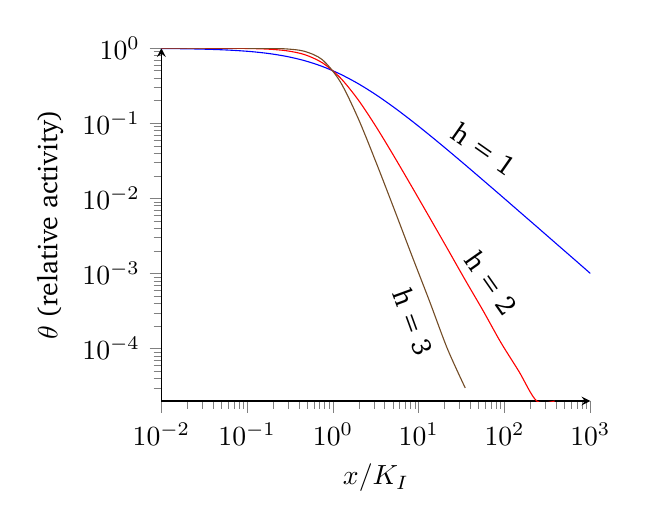
\begin{tikzpicture}
	\begin{loglogaxis}[width=200pt,axis x line=bottom, axis y line=left, tick align=outside, domain=1e-2:1e3, xlabel=$x/K_I$, ylabel=$\theta$ (relative activity)]
		\addplot+[mark=none,smooth] (\x,{(1 - (\x/(1+\x))});
		\addplot+[mark=none,smooth] (\x,{(1 - (\x^2/(1+\x^2))});
		\addplot+[mark=none,smooth] (\x,{(1 - (\x^3/(1+\x^3))});
		\end{loglogaxis}
	\node[rotate=-35] at (4.1, 3.2) {h = 1};
	\node[rotate=-55] at (4.2, 1.5) {h = 2};
	\node[rotate=-70] at (3.2, 1) {h = 3};
\end{tikzpicture}
\end{center}

In this case, the elasticity with regards to the inhibitor concentration would be:
\begin{eqnarray}
    \varepsilon_x^v &=& \frac{\partial v}{\partial x}\cdot\frac{x}{v} = V^+ ~ \kappa ~ \gamma ~ \frac{- h ~ x^{h-1}}{(K_I^h + x^h)^2} ~ \frac{x}{v} \nonumber \\
    &=& -\frac{h ~ x^h ~ (K_I^h + x^h)}{(K_I^h + x^h)^2} = -h ~ \frac{x^h}{K_I^h + x^h} = -h (1 - \theta)~. \label{eq:eps_inh}
\end{eqnarray}

Plotting the elasticity as a function of $x$, we see that it is a monotonically decreasing negative function:

\begin{center}
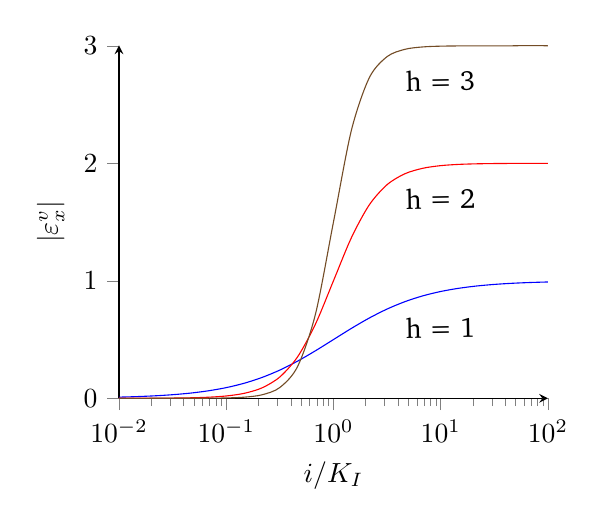
\begin{tikzpicture}
\begin{semilogxaxis}[width=200pt,axis x line=bottom, axis y line=left, tick align=outside, domain=1e-2:1e2, xlabel=$i/K_I$, ylabel=$|\varepsilon_x^v|$]
		\addplot+[mark=none,smooth] (\x,{1 * (\x/(1+\x))});		\addplot+[mark=none,smooth] (\x,{2 * (\x^2/(1+\x^2))});		\addplot+[mark=none,smooth] (\x,{3 * (\x^3/(1+\x^3))});
	\node[rotate=1] at (10, 0.6) {h = 1};
	\node[rotate=1] at (10, 1.7) {h = 2};
	\node[rotate=1] at (10, 2.7) {h = 3};
	\end{semilogxaxis}
\end{tikzpicture}
\end{center}

This means that substrates have the most control ($|\varepsilon_s^v| \rightarrow 1$) when they are much below saturation ($s \ll K_M$) while inhibitors have the most control ($|\varepsilon_x^v| \rightarrow h$) when they are saturated ($x \gg K_I$).


\subsubsection{Competitive Inhibition}
Competitive inhibition is one case, where a separable kinetic rate law is not sufficient since $\frac{\partial \kappa}{\partial x} \neq 0$. To analyze this case, we pick a simple one-substrate irreversible reaction, where the inhibitor affects the $K_M$ according to the following formula:
\begin{eqnarray}
    v &=& V^+ ~ \frac{s}{K_M \left(1 + \frac{x^h}{K_I^h}\right) + s}
\end{eqnarray}
In this case, we can define an \emph{effective} inhibition constants $K_{IC}$, that will allow us to rewrite this rate law in a form identical to non-competitive inhibition:
\begin{eqnarray}
    K_{IC} &\equiv& K_I \sqrt[h]{\frac{K_M + s}{K_M}} \nonumber\\
    v &=& V^+ ~ \frac{s}{K_M \left(1 + \frac{x^h}{K_I^h}\right) + s} =
          V^+ ~ \frac{s}{K_M \left(1 + \frac{x^h~(K_M + s)}{K_{IC}^h~K_M}\right) + s} = \nonumber\\
      &=& V^+ ~ \frac{s}{K_M + s + \frac{x^h~(K_M + s)}{K_{IC}^h}} = 
          V^+ ~ \frac{s}{K_M + s} \cdot \frac{1}{1 + \frac{x^h}{K_{IC}^h}} \label{eq:eps_comp_inh}
\end{eqnarray}
so we can see here that in this case $\theta = \frac{K_{IC}^h}{K_{IC}^h~+~x^h}$, exactly like in the case of non-competitive inhibition. Of course, the difference here is that $K_{IC}$ is not a binding constant but rather a function of $s$, $K_M$, and $K_I$. Nevertheless, we can use the same formula for the elasticity (since $K_{IC}$ is a constant with regards to $x$):
\begin{eqnarray}
    \varepsilon_x^v &=& \frac{\partial v}{\partial x}~\frac{x}{v} = -h(1 - \theta)\,.
\end{eqnarray}
Note, that since $K_{IC} > K_I$, then also $\theta$ in this case is larger (closer to $1$) than the equivalent value of the inhibition term in the non-competitive case, and thus $\varepsilon_x^v$ would be higher (closer to zero). Therefore, assuming non-competitive inhibition by default would be an overestimate of the absolute elasticity $|\varepsilon_x^v|$.

Unlike for the case of pure non-competitive inhibition, where $\theta$ is a multiplicative term in the rate law, a competitive inhibition also affects the elasticity of the substrate:
\begin{eqnarray}
\varepsilon_{s}^v &=& 1 - \frac{s}{K_M \left(1 + \frac{x^h}{K_I^h}\right)+ s} < 1 - \frac{s}{K_M + s}
\end{eqnarray}
Therefore, as is the case for reversible reactions (Equation \ref{eq:reversible_substrate_eps}), the substrate elasticity would be higher than the simple irreversible elasticity -- i.e. it would be underestimated.

\subsubsection{Product Inhibition}
It is often the case, that the product of a reaction also acts as a competitive inhibitor, i.e. following this rate law:
\begin{eqnarray}
v &=& V^+ ~ \frac{s}{K_S \left(1 + \frac{p^h}{K_P^h}\right) + s}\,.
\end{eqnarray}
The product and substrate elasticities would thus follow exactly the case analyzed in the previous section, except for the product $p$ instead of an inhibitor $x$.

\subsubsection{Uncompetitive Inhibition}
Uncompetitive inhibition is another case where substrate and inhibitor saturations are entangled:
\begin{eqnarray}
    v &=& V^+ ~ \frac{s}{K_M + s \left(1 + \frac{x^h}{K_I^h}\right)}
\end{eqnarray}
However, the same procedure as in competitive inhibition can also be used here, by defining an effective constant $K_{IU}$, that will allow us to rewrite this rate law in a form identical to non-competitive inhibition:
\begin{eqnarray}
    K_{IU} &\equiv& K_I \sqrt[h]{\frac{K_M + s}{s}} \nonumber\\
    v &=& V^+ ~ \frac{s}{K_M + s \left(1 + \frac{x^h}{K_I^h}\right)} =
          V^+ ~ \frac{s}{K_M + s \left(1 + \frac{x^h~(K_M + s)}{K_{IU}^h~s}\right)} = \nonumber\\
      &=& V^+ ~ \frac{s}{K_M + s + \frac{x^h~(K_M + s)}{K_{IU}^h}} = 
          V^+ ~ \frac{s}{K_M + s} \cdot \frac{1}{1 + \frac{x^h}{K_{IU}^h}}
\end{eqnarray}
which shows that just like in the case of competitive inhibition, $\theta = \frac{K_{IU}^h}{K_{IU}^h~+~x^h}$, and the formula for elasticity remains
\begin{eqnarray}
    \varepsilon_x^v = -h(1 - \theta)\,. \label{eq:eps_uncomp_inh}
\end{eqnarray}

\subsubsection{Generalized Inhibition Model}
A general formula for reversible reactions with non-cooperative competitive, uncompetitive, mixed and pure non-competitive inhibition is given in Chapter 5 of \citet{Sauro2011-op}:
\begin{eqnarray}\label{eq:gen_inh_model}
    v &=& \frac{\frac{V^+}{K_S}\left(s - \frac{p}{K_{eq}}\right)\left(1 + b \frac{x}{aK_I}\right)}{\left(1 + \frac{s}{K_S} + \frac{p}{K_P}\right) + \frac{x}{K_I} \left(1 + \frac{s}{aK_S} + \frac{p}{aK_P}\right)}\,.
\end{eqnarray}
The parameter $b$ represents the amount of inhibition, i.e. the activity of the enzyme when the inhibitor is bound to it. If we assume there is no activity in the bound state, also known as \textbf{complete inhibition}, then we can set $b = 0$. 
Then, depending on the value of $a$, the above formula converges to the different cases discussed earlier. For example, if $a \rightarrow \infty$, then this rate law is equivalent to competitive inhibition. When $a = 1$ it is equivalent to pure non-competitive inhibition. Finally, if $a \rightarrow 0$ (more precisely, when $K_I \gg a K_I$), it becomes uncompetitive inhibition.

The elasticity we get for this general form is:
\begin{eqnarray}
\varepsilon_x^v &=& \frac{b \frac{x}{aK_I}}{1 + b \frac{x}{aK_I}} ~-~ \frac{\frac{x}{K_I} \left(1 + \frac{s}{aK_S} + \frac{p}{aK_P}\right)}{\left(1 + \frac{s}{K_S} + \frac{p}{K_P}\right) + \frac{x}{K_I} \left(1 + \frac{s}{aK_S} + \frac{p}{aK_P}\right)}
\end{eqnarray}
as with previous cases, we can define an effective $K_E$:
\begin{eqnarray}
    K_{E1} & \equiv & K_I ~ \frac{a}{b} \\
    K_{E2} & \equiv & K_I ~ \frac{1 + \frac{s}{K_S} + \frac{p}{K_P}}{1 + \frac{s}{aK_S} + \frac{P}{aK_P}}
\end{eqnarray}
and therefore that we rewrite the rate law from Eq. \ref{eq:gen_inh_model} as:
\begin{eqnarray}
\kappa &\equiv& \frac{1}{K_S \left(1 + \frac{s}{K_S} + \frac{p}{K_P}\right)} \nonumber \\
\gamma &\equiv& s - \frac{p}{K_{eq}} \nonumber \\
\theta &\equiv& \frac{1 + \frac{x}{K_{E1}}}{1 + \frac{x}{K_{E2}}} \nonumber \\
v &=& V^+ \cdot \kappa \cdot \gamma \cdot \theta
\end{eqnarray}
The elasticity thus becomes:
\begin{eqnarray}
\varepsilon_x^v &=& 
	\frac{\frac{x}{K_{E1}}}{1 + \frac{x}{K_{E1}}} ~-~ \frac{\frac{x}{K_{E2}}}{1 + \frac{x}{K_{E2}}} = 
	\left( 1 - \frac{1}{1 + \frac{x}{K_{E1}}} \right) ~-~ \left(1 - \frac{1}{1 + \frac{x}{K_{E2}}} \right) \nonumber\\
	&=& -\left(\frac{1}{1 + \frac{x}{K_{E1}}} -  \frac{1}{1 + \frac{x}{K_{E2}}} \right) = 
	-\left( 1 -  \frac{1 + \frac{x}{K_{E1}}}{1 + \frac{x}{K_{E2}}} \right) \cdot \frac{1}{1 + \frac{x}{K_{E1}}} \nonumber\\
	&=& -(1 - \theta) \cdot  \frac{1}{1 + \frac{x}{K_{E1}}}
\end{eqnarray}
and after replacing $K_{E1}$ back with its definition:
\begin{eqnarray}
	\varepsilon_x^v = -\left(1 - \theta\right) \cdot  \left( 1 + b \frac{x}{aK_I} \right)^{-1}
\end{eqnarray}

As expected, in all cases of complete inhibition ($b = 0$), we reach exactly the same conclusion as in the extreme cases, namely:
\begin{eqnarray}
\varepsilon_x^v = -(1 - \theta) \label{eq:eps_general_inh}
\end{eqnarray}

\subsubsection{The Monod-Changeux-Jacob model}
Probably the most widespread model for cooperativity of substrate and effector binding was proposed by \citet{Monod1965-dq}. In this model the rate law is given by the following formula:
\begin{eqnarray}
v &=& V^+ \cdot \frac{s}{K_M + s} \cdot \frac{\left(1 + \frac{s}{K_M}\right)^h \left(1 + \frac{a}{K_A}\right)^h \left(1 + \frac{x}{K_I}\right)^{-h}}{L + \left(1 + \frac{s}{K_M}\right)^h \left(1 + \frac{a}{K_A}\right)^h \left(1 + \frac{x}{K_I}\right)^{-h}}
\end{eqnarray}
where $a$ is the concentration of an inhibitor, and $K_M$, $K_A$ and $K_I$ are the dissociation constants for the active form of the enzyme (for $s$, $a$ and $x$ respectively), $n$ is the number of subunits, and $L$ is the allosteric constant. As before, we can define the saturation term $\kappa$ and the relative activity term $\theta$ (i.e. the decrease from maximal activity):
\begin{eqnarray}
\kappa &\equiv& \frac{s}{K_M + s} \nonumber\\
\theta &\equiv& \frac{\left(1 + \frac{s}{K_M}\right)^h \left(1 + \frac{a}{K_A}\right)^h \left(1 + \frac{x}{K_I}\right)^{-h}}{L + \left(1 + \frac{s}{K_M}\right)^h \left(1 + \frac{a}{K_A}\right)^h \left(1 + \frac{x}{K_I}\right)^{-h}} \nonumber\\
v &=& V^+ \cdot \kappa \cdot \theta
\end{eqnarray}
To simplify the form of the equations, let 
\begin{equation}
g(x) \equiv \left(1 + \frac{s}{K_M}\right)^h \left(1 + \frac{a}{K_A}\right)^h \left(1 + \frac{x}{K_I}\right)^{-h}
\end{equation}

\noindent so that $\theta = \frac{g(x)}{L + g(x)}$, which we write in shorthand as $\theta= \frac{g}{L+g}$. Then, 
\begin{eqnarray}
\varepsilon_x^v = V^+ \cdot \kappa \cdot \frac{\partial\theta}{\partial x} \cdot \frac{x}{v} 
= V^+ \cdot \kappa \cdot \frac{L}{(L+g)^2} \cdot \frac{\partial g}{\partial x} \cdot \frac{x}{v}
\end{eqnarray}

Now, we can calculate that 
\begin{equation}
\frac{\partial g}{\partial x} = \frac{-h}{K_I + x} \cdot g
\end{equation}

Substituting this form of $\frac{\partial g}{\partial x}$ into the prior equation, we arrive at 
\begin{eqnarray}
\varepsilon_x^v = V^+ \cdot \kappa \cdot \frac{g}{L + g} \cdot \frac{-hx}{K_I + x} \cdot \frac{L}{L + g} \cdot \frac{1}{v}
\end{eqnarray}

\noindent Note that the first three terms are precisely equal to $v$, so they cancel with the last term. Also note that $\frac{L}{L + g} = 1 - \frac{g}{L + g} = 1 - \theta$. Thus, we arrive at

\begin{eqnarray}
\varepsilon_x^v = \frac{\partial \ln{v}}{\partial \ln{x}} = \frac{\partial \ln{\theta}}{\partial \ln{x}} = -h~\frac{x}{K_I + x} ~\left(1 - \theta \right)\,.
\end{eqnarray}

In \cite{Heinrich1974-yj}, the elasticity of the inhibitor was calculated for this rate law (denoted as \emph{effector strength} or $X_I$ in the original text) and matches the form above.
Although the final formulae for the elasticities in the MWC case are not identical to the other cases dealt with before, we can still reach a similar conclusion, where the absolute value of the elasticity is larger when the relative activity is smaller.

\subsection{Multi-substrate Reactions}
So far, we focused only on reactions that have a single substrate. Below, we calculate elasticities for multi-substrate reactions (with substrates $s_1 \ldots s_n$), assuming general irreversible convenience kinetics with a pure non-competitive inhibitor, namely
\begin{eqnarray}
v &=& V^+ \cdot \kappa \cdot \theta  \nonumber\\
\kappa &=& \frac{\prod_i s_i/K_i}{\prod_i (1 + s_i/K_i) - 1}\,.
\end{eqnarray}

Here, the elasticity with respect to the inhibitor is a separate multiplicative factor and therefore is exactly the same as in section \ref{sec:non_conpetitive_inhitibion}. Calculating the elasticity of substrate $s_i$, we get 
\begin{eqnarray}
\varepsilon^{v}_{s_j} &=& \frac{\partial v}{\partial s_j} \cdot \frac{s_j}{v}
 = \frac{\partial \kappa}{\partial s_j} \cdot \frac{s_j}{\kappa} 
 = \frac{\prod_{i \neq j}(1 + s_i/K_i) - 1}{\prod_j (1 + s_i/K_i) - 1} \nonumber\\
 &=& 1 - \left(s_j/K_j\right) \cdot \frac{\prod_{i \neq j} (1 + s_i/K_i)}{\prod_i (1 + s_i/K_i) - 1} \nonumber \\
 &=& 1 - \frac{ s_j/K_j}{1 +  s_j/K_j} \cdot \left(\frac{\prod_i (1 + s_i/K_i)}{\prod_i (1 + s_i/K_i) - 1}\right) 
 \,.
\end{eqnarray}

In order to compare this result to the mono-substrate case, we first note that the multiplicative term (in parentheses) is larger than 1 since the denominator is obviously smaller than the numerator. Therefore:
\begin{eqnarray}
\varepsilon^{v}_{s_j} < 1 -  \frac{ s_j/K_j}{1 +  s_j/K_j} = 1 - \frac{ s_j}{K_j +  s_j}\,
\end{eqnarray}
which is exactly the expression for the substrate elasticity in the case of mono-substrate irreversible reactions (Equation \ref{eq:eps_s_v_irr}). Thus, we conclude that the mono-substrate reaction scheme is an over-estimate of the true elasticity in a multi-substrate reaction scheme (following convenience kinetics).

\subsection{A Trade-off between Enzyme Cost and Flux Control}
By taking the absolute value of the elasticity, we can compress the results for activators (Equation \ref{eq:eps_act}) and inhibitors (Equations \ref{eq:eps_inh}, \ref{eq:eps_comp_inh}, \ref{eq:eps_uncomp_inh}, and \ref{eq:eps_general_inh}, excluding the MWC model) into one formula:
\begin{eqnarray}
|\varepsilon_x^v| = h (1 - \theta)~. \label{eq:abs_elast}
\end{eqnarray}
This relationship can be visualized in the following plot (for different values of $h$):
\begin{center}
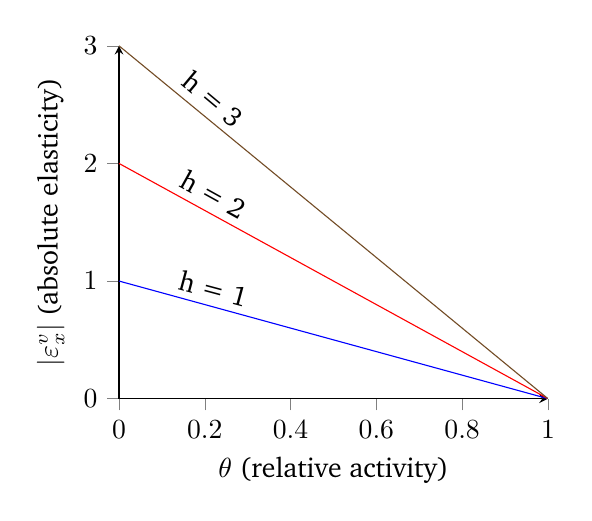
\begin{tikzpicture}[scale=1]
	\begin{axis}[width=200pt,axis x line=bottom, axis y line=left, tick align=outside, domain=0:1, xlabel=$\theta$ (relative activity), ylabel=$|\varepsilon_x^v|$ (absolute elasticity)]
		\addplot+[mark=none,smooth] (\x,{1 * (1 - \x)});
		\addplot+[mark=none,smooth] (\x,{2 * (1 - \x)});
		\addplot+[mark=none,smooth] (\x,{3 * (1 - \x)});
	\end{axis}
	\node[rotate=-15] at (1.2, 1.4) {h = 1};
	\node[rotate=-29] at (1.2, 2.6) {h = 2};
	\node[rotate=-40] at (1.2, 3.8) {h = 3};
\end{tikzpicture}
\end{center}

Since $\theta$ represents the fraction of active enzyme, we see here that there is direct trade-off between the activity of the enzyme and the elasticity. It should be noted, that evolution can easily adjust $\theta$ for an individual enzyme by changing the $K_A$ or $K_I$ values, even without changing the concentration of the small-molecule effector (assuming it has other crucial functions in the cell). Therefore, evolution needs to weigh between how much of the enzyme is "wasted" by inhibition (or by inactivation), versus how much control it has on the flux. This can be viewed as a trade-off between the short-term goal of being able to adjust things quickly and the long-term goal of allocating resources efficiently in order to grow as fast as possible.

Another corollary of Equation \ref{eq:abs_elast} is that the control can be increased by changing the Hill coefficient ($h$). This could be a reason why mechanisms with very high cooperativity evolve for allosteric regulation \cite{Monod1965-dq}, as it increases elasticity without the added cost of losing enzyme activity.

\addcontentsline{toc}{section}{References}
\bibliographystyle{unsrtnat}
\bibliography{control_theory}
\clearpage

\section{Supplementary Figures}

\begin{figure}[ht!]
\begin{center}
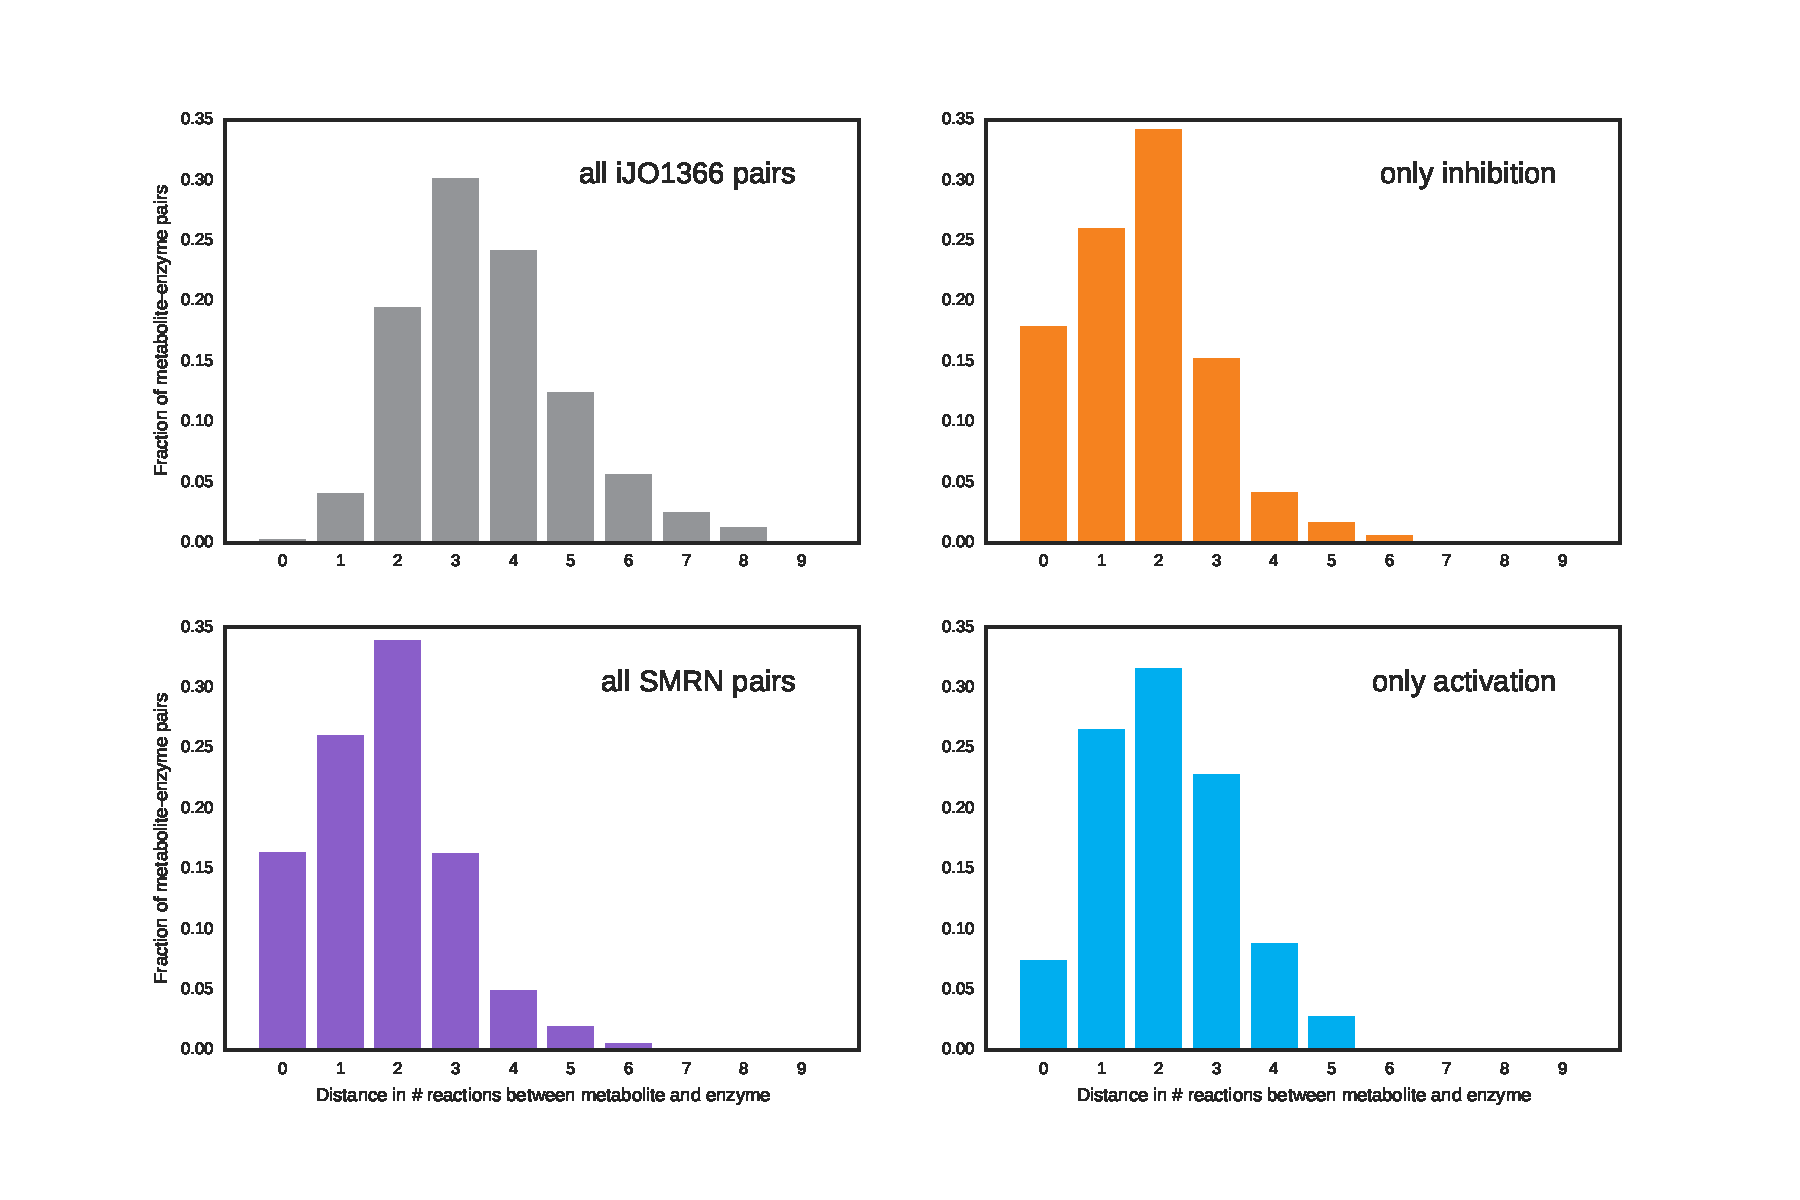
\includegraphics[width=0.85\textwidth]{../manuscript/figS1.pdf}
\end{center}
\caption{Distance between metabolites and enzymes in the (a) genome-scale metabolite network iJO1366 and (b)-(d) the SMRN of E. coli. In general, interactions in the SMRN traverse a shorter distance than the typical distance between a randomly chosen metabolite and enzyme in metabolism. Several highly-connected metabolites (i.e. co-factors) that were removed from the network before preparing the bipartite graph: h, h2o, co2, o2, pi, atp, adp, amp, nad, nadh, nadp, nadph, coa, thf, 5mthf, 5fthf, methf, mlthf, nh4, cmp, q8, q8h2, udp, udpg, fad, fadh2, ade, ctp, gtp, h2o2, mql8, mqn8, na1, ppi, acp. Histogram of the number of interactions for reactions and metabolite in the (e)-(f) entire \emph{E. coli} SMRN, and (g)-(h) in the region of the SMRN restricted to the central carbon metabolism (CCM) of E. coli. }
\end{figure}

\begin{figure}[ht!]
	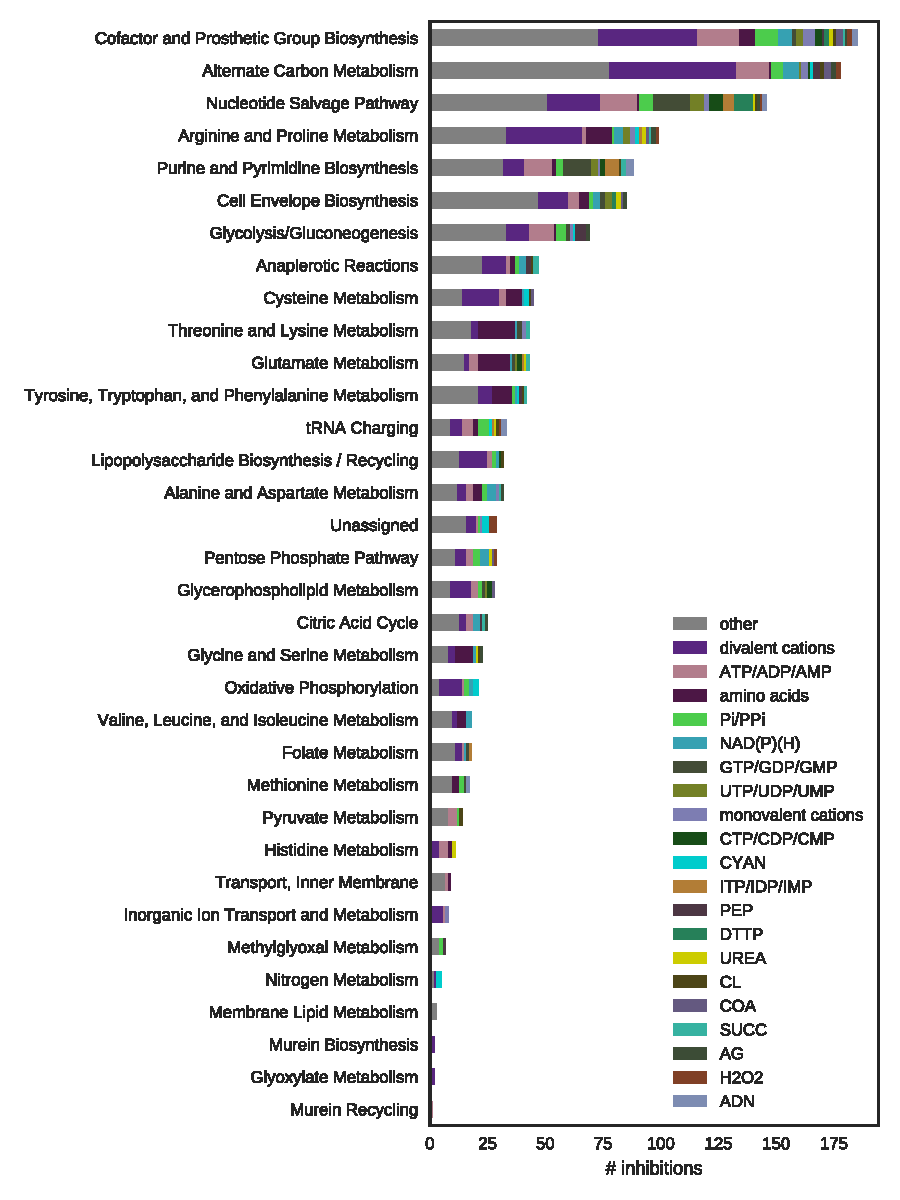
\includegraphics[width=\textwidth]{../manuscript/figS3.pdf}
	\caption{Number of interactions in the SMRN targeting each pathway in E. coli metabolism. 
	}
\end{figure}

\begin{figure}[ht!]
	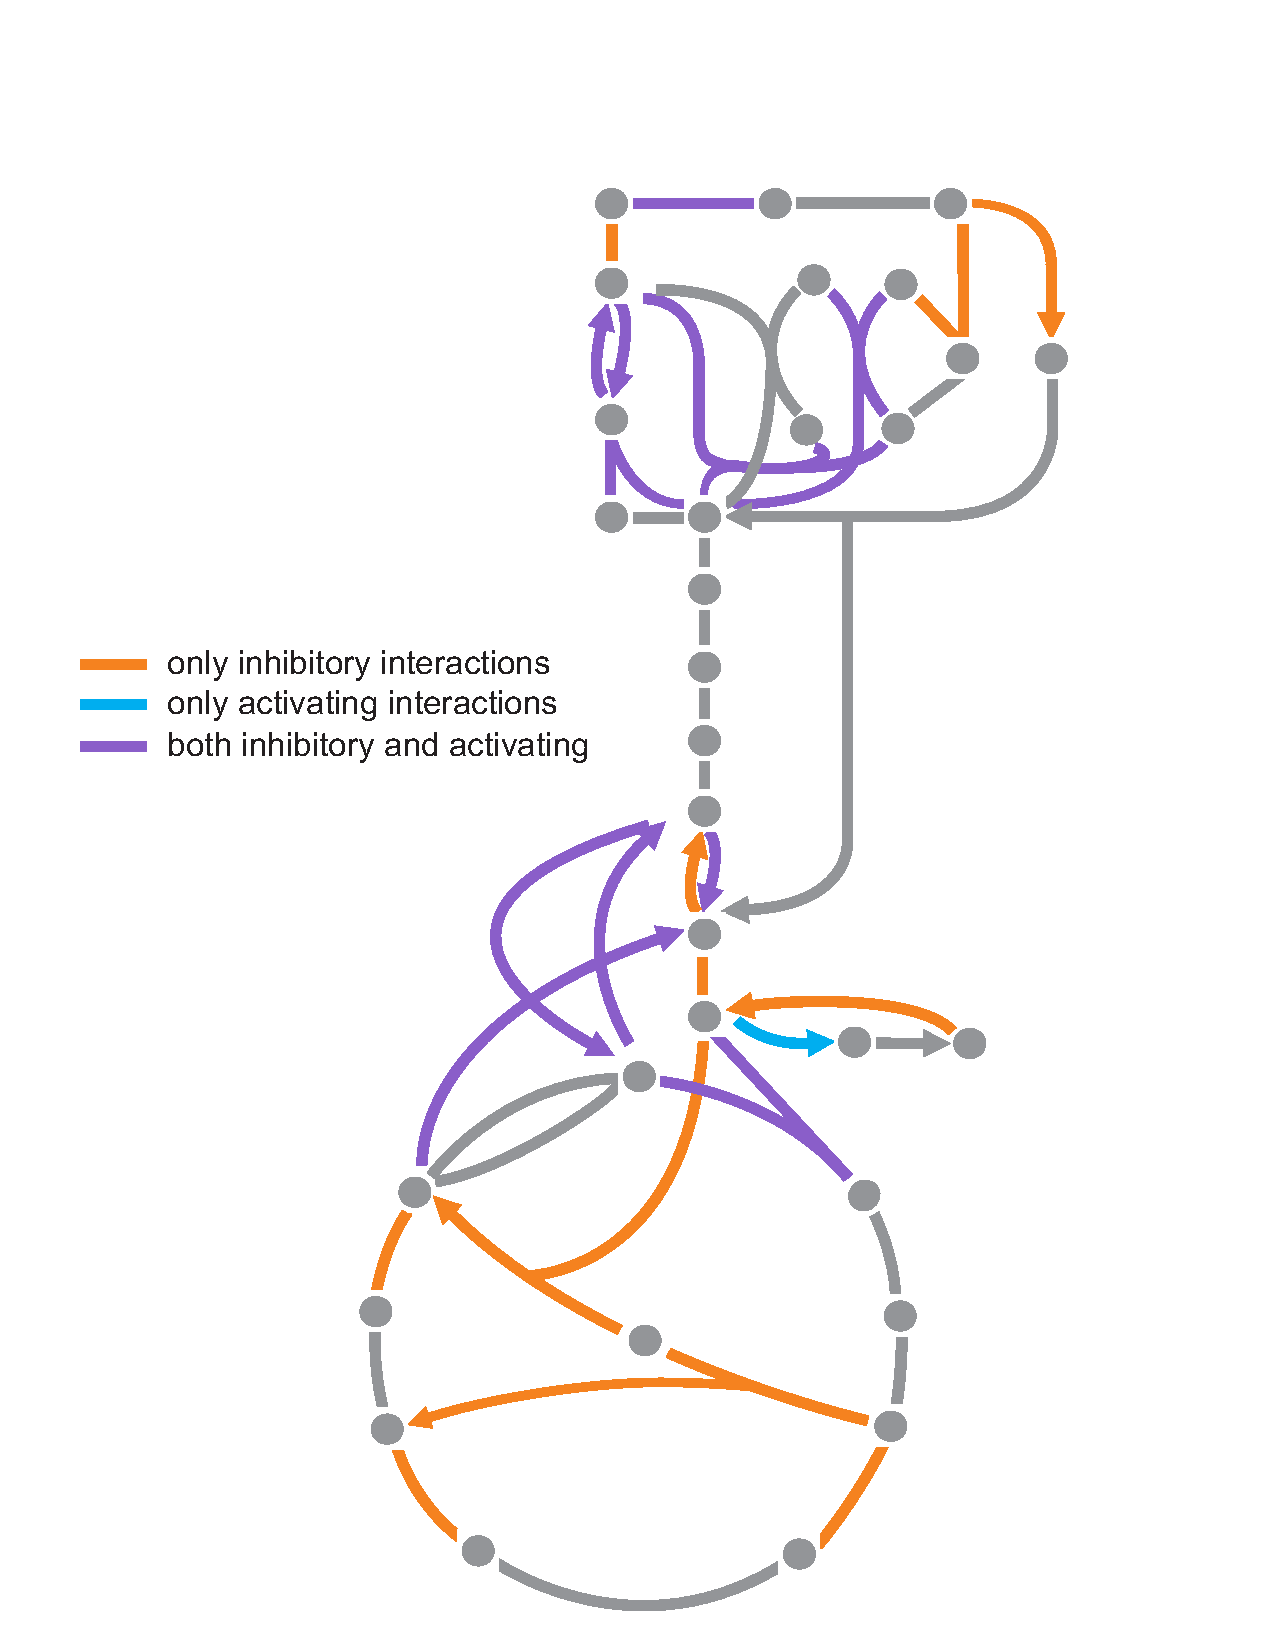
\includegraphics[width=\textwidth]{../manuscript/figS8.pdf}
	\caption{A map of the Central Metabolism reactions in \emph{E. coli} that are regulated by small molecule(s) in the SMRN. Red reactions only show evidence of inhibitory interactions, green reactions only show evidence of activating interactions, and purple reactions show evidence of both activating and inhibiting interactions. 
	}
\end{figure}

\begin{figure}[ht!]
	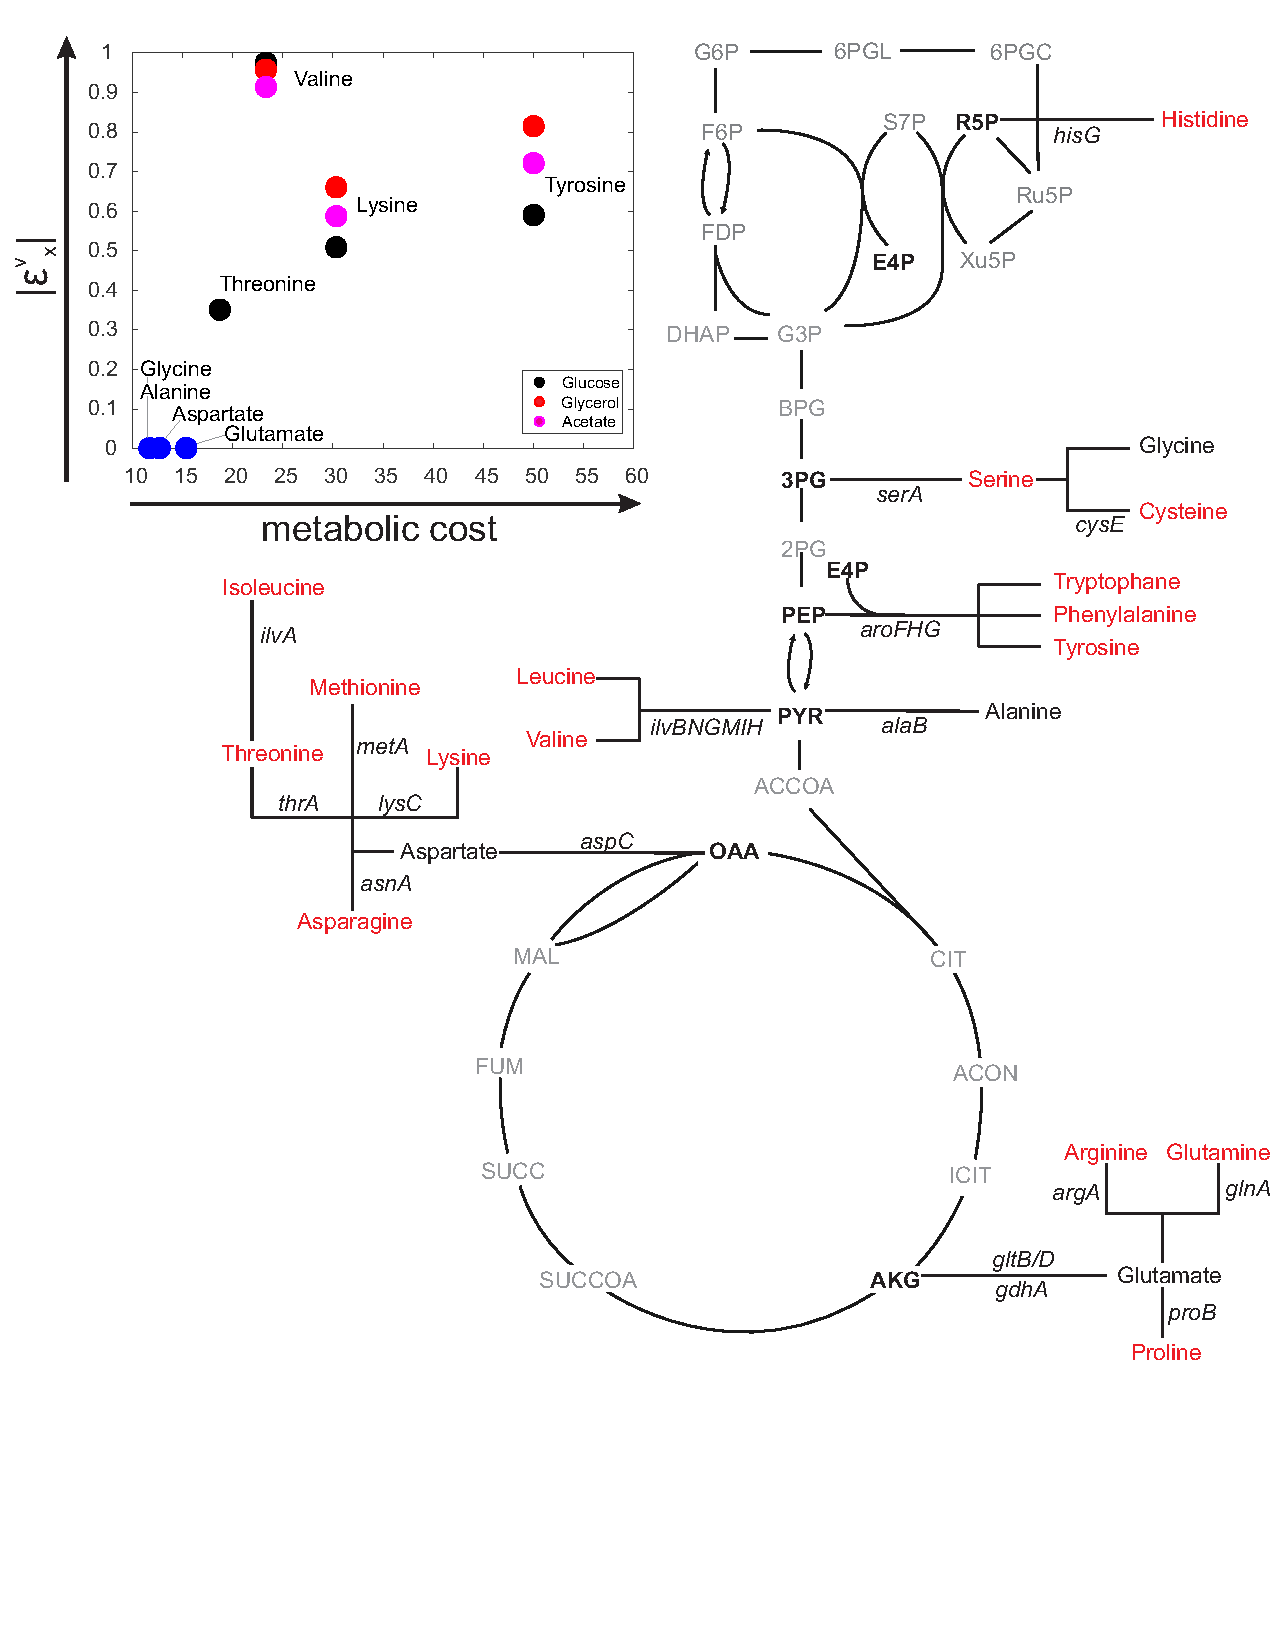
\includegraphics[width=0.9\textwidth]{../manuscript/FigureS4new.pdf}
	\caption{A map of the reactions branching from central carbon metabolism for amino acid biosynthesis. Amino acids in red color feedback inhibit the first enzyme of their biosynthesis pathway, based on the SMRN. For the remaining four amino acids (Glycine, Alanine, Aspartate and Glutamate) there is no evidence of feedback inhibition. In the inset on the top-left corner, we present a comparison between the metabolic cost of each amino acid (as defined by \cite{Akashi2002-ew}) and the absolute elasticity of the corresponding inhibited biosynthetic reaction (if it exists) for three growth conditions. We only have information for 4 of the 16 regulated biosynthetic pathways. All four non-regulated amino-acids were assumed to have 0 elasticity (marked in blue).}\label{fig:SI_biosynthesis}
\end{figure}

\begin{figure}[ht!]
	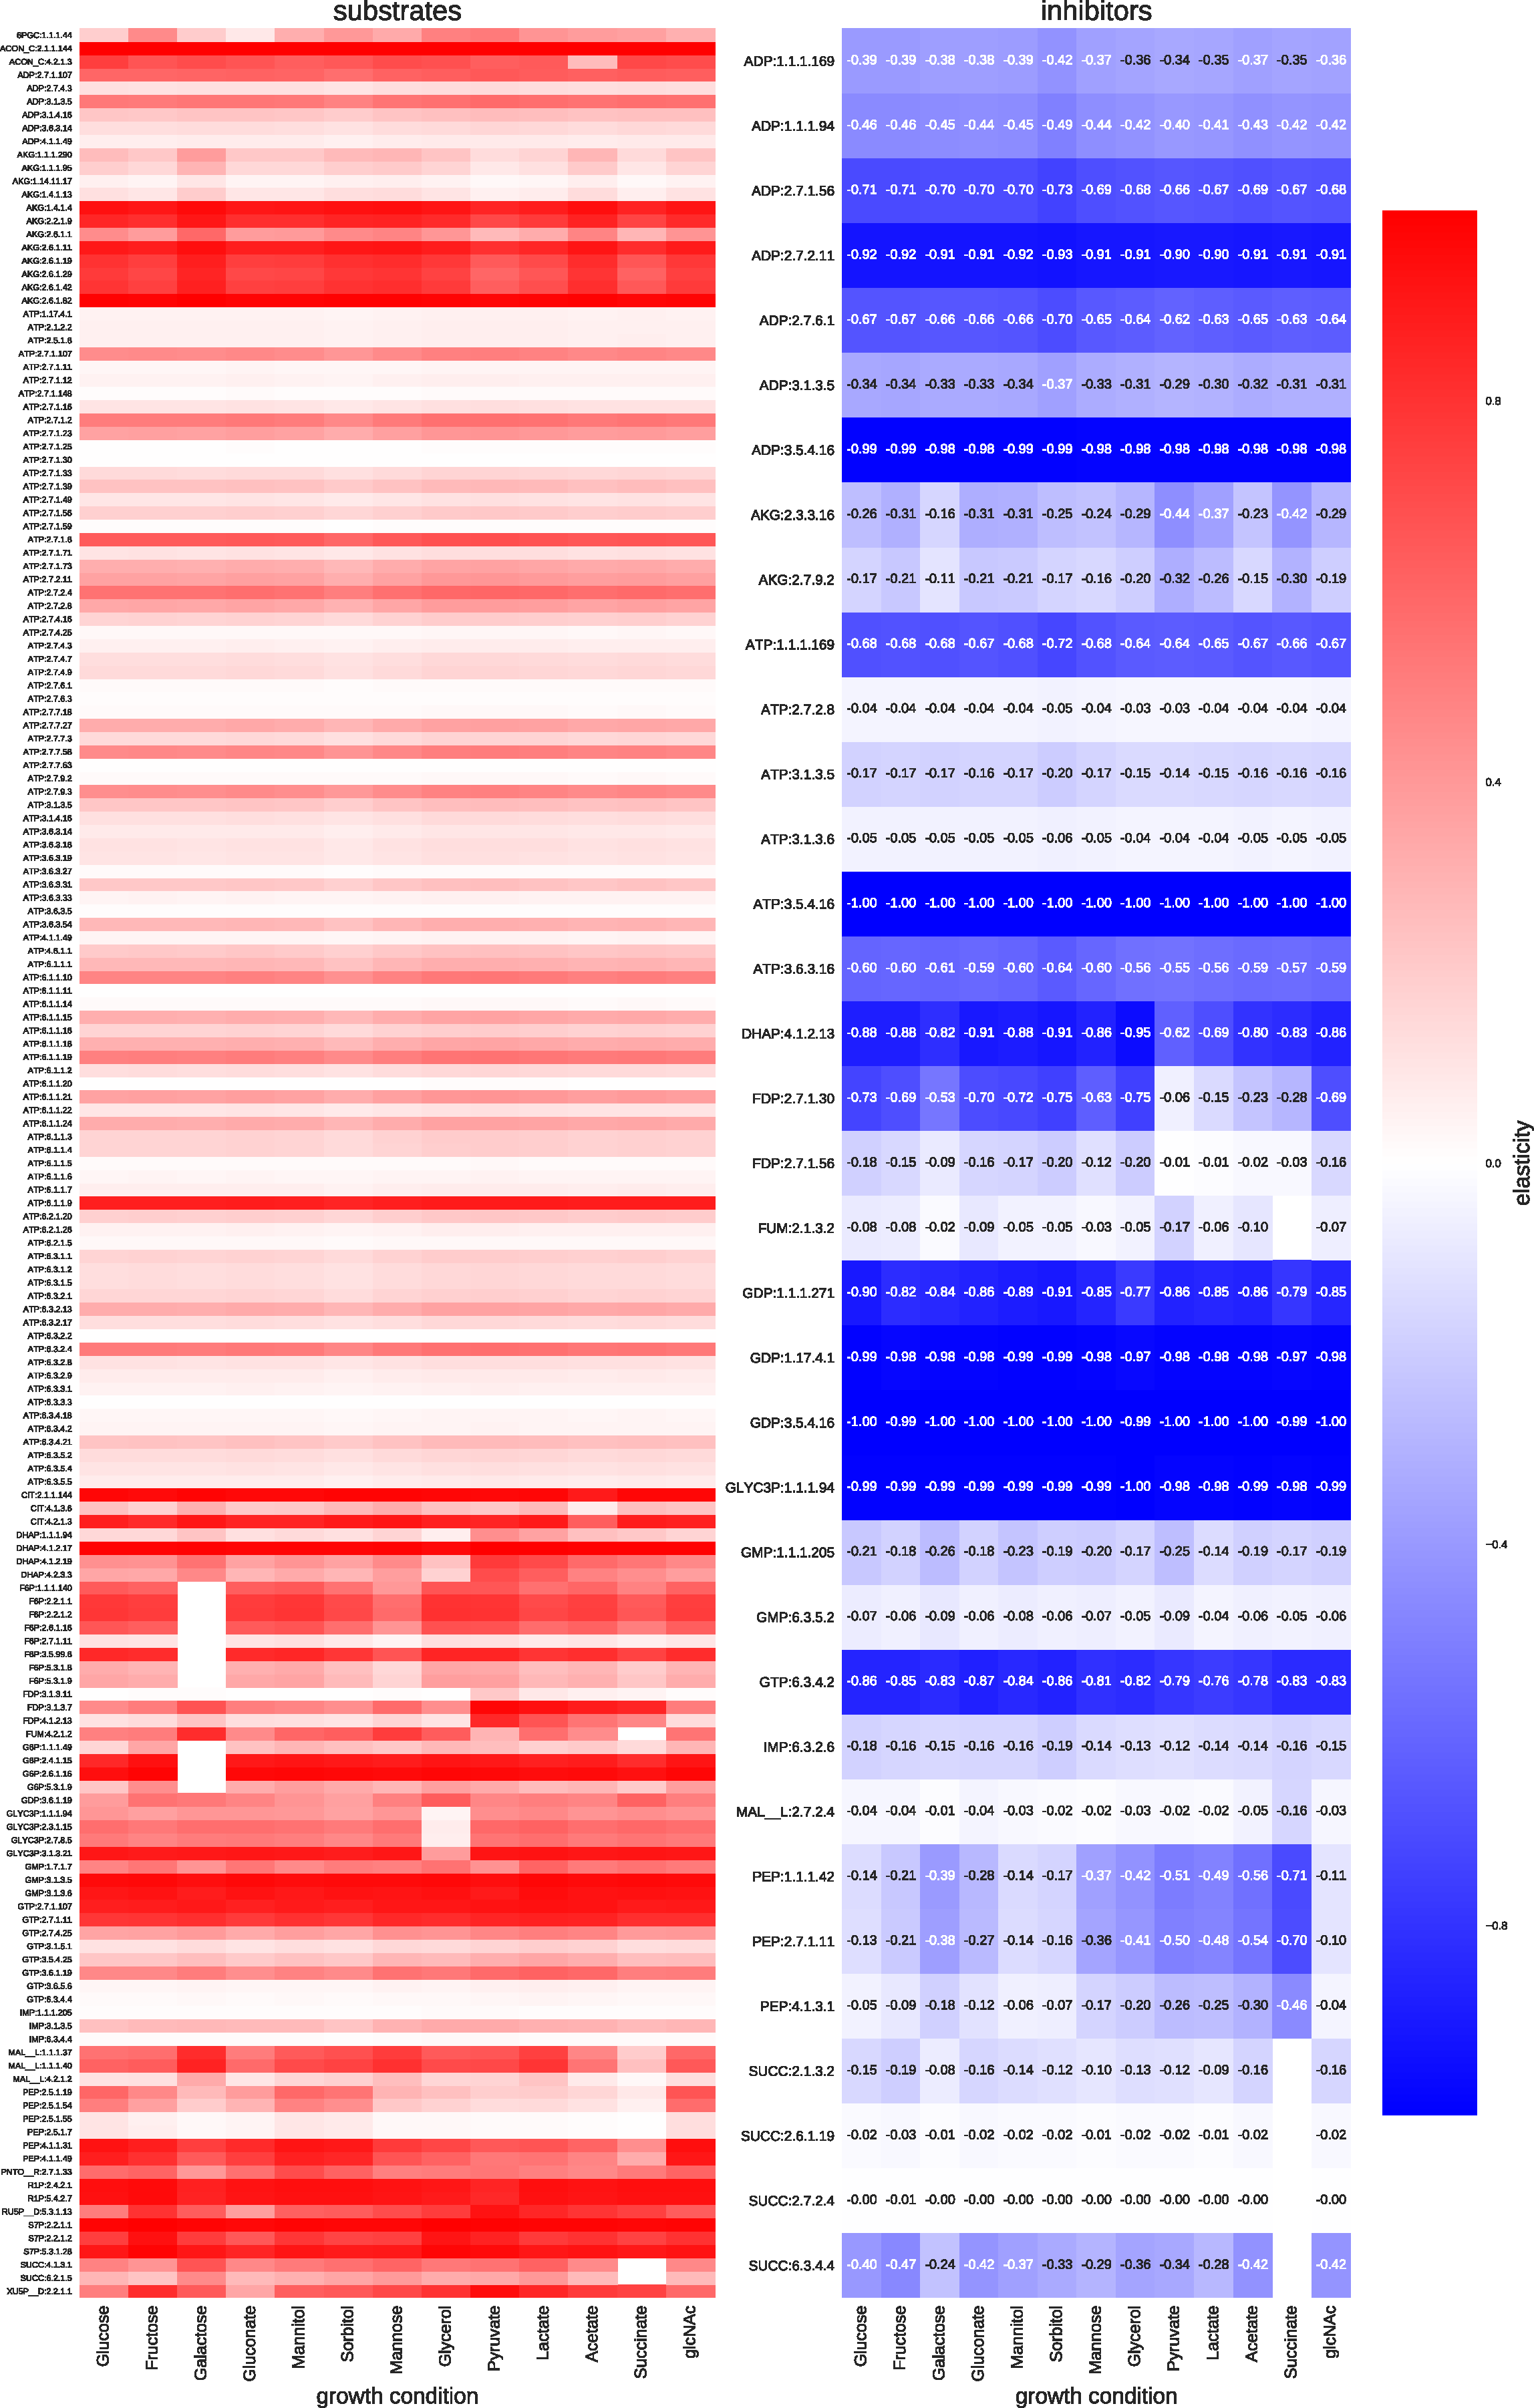
\includegraphics[width=1.1\textwidth]{../manuscript/figS4.pdf}
	\caption{Schematic of the relationship between kinetic rate laws and elasticity for (a)-(b) substrates obeying Michaelis-Menten kinetics and (c)-(d) inhibitors obeying non-competitive inhibition. Importantly, substrate elasticity is maximized at low substrate concentrations, and inhibitor elasticity is maximized at high inhibitor concentration.
	}
\end{figure}

\begin{figure}[ht!]
	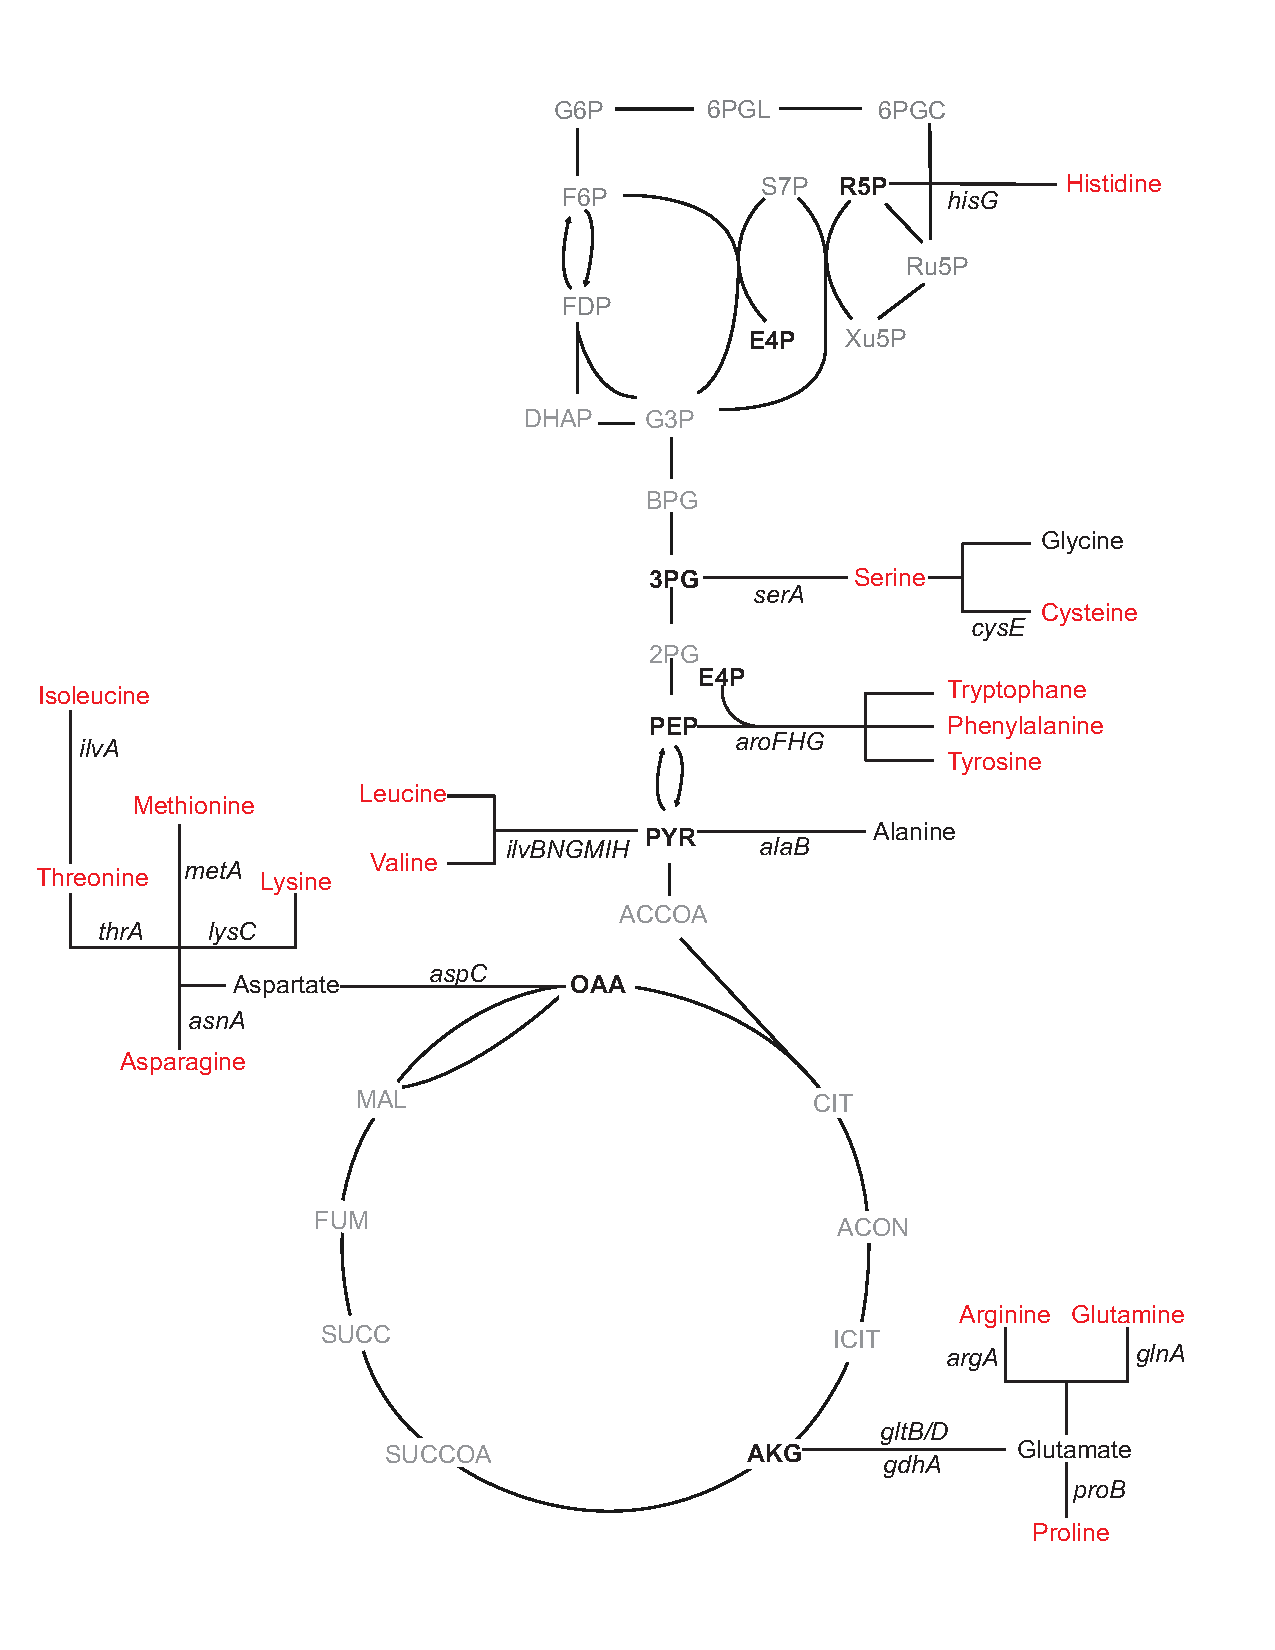
\includegraphics[width=\textwidth]{../manuscript/figS6.pdf}
	\caption{For 45 metabolites, we were able to obtain 2 or more estimates each of KM and KI values. This enabled us to directly compare, on a single-metabolite basis, whether the distributions of its KM and KI values differed substantially. Doing so, we found that 5 metabolites (PEP, ATP, methionine, succinate, and dGMP) each showed significantly higher values of KI values compared to KM values (FDR-adjusted Mann-Whitney p-value < 0.1) and only one metabolite (phosphate) had significantly lower KI values.
	}
\end{figure}

%\begin{figure}[ht!]
%	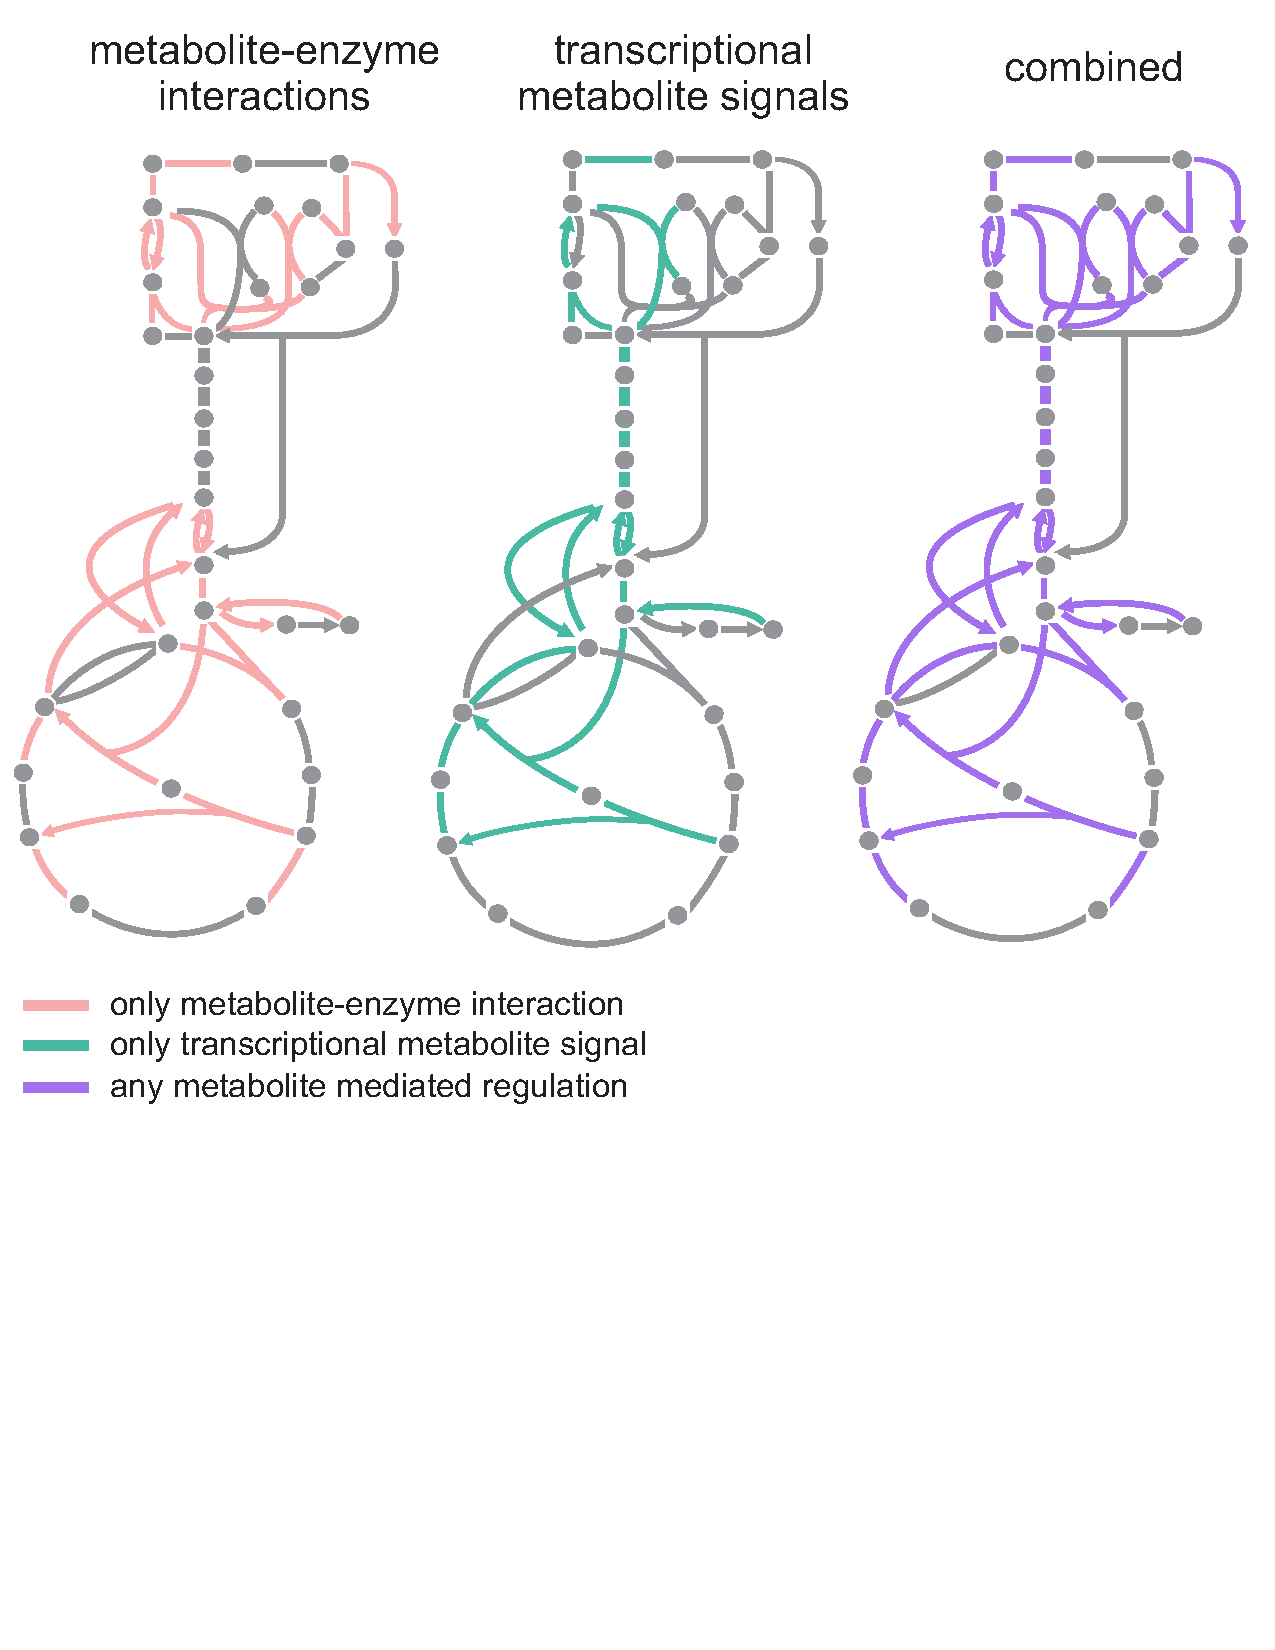
\includegraphics[width=0.8\textwidth]{../manuscript/figS5.pdf}
%	\caption{A heatmap of the median values of each metabolite's elasticities across a variety of nutrient conditions. Left-hand-side corresponds to substrate interactions for that metabolite, and right-hand-side corresponds to inhibitory interactions.
%	}
%\end{figure}

\begin{figure}[ht!]
	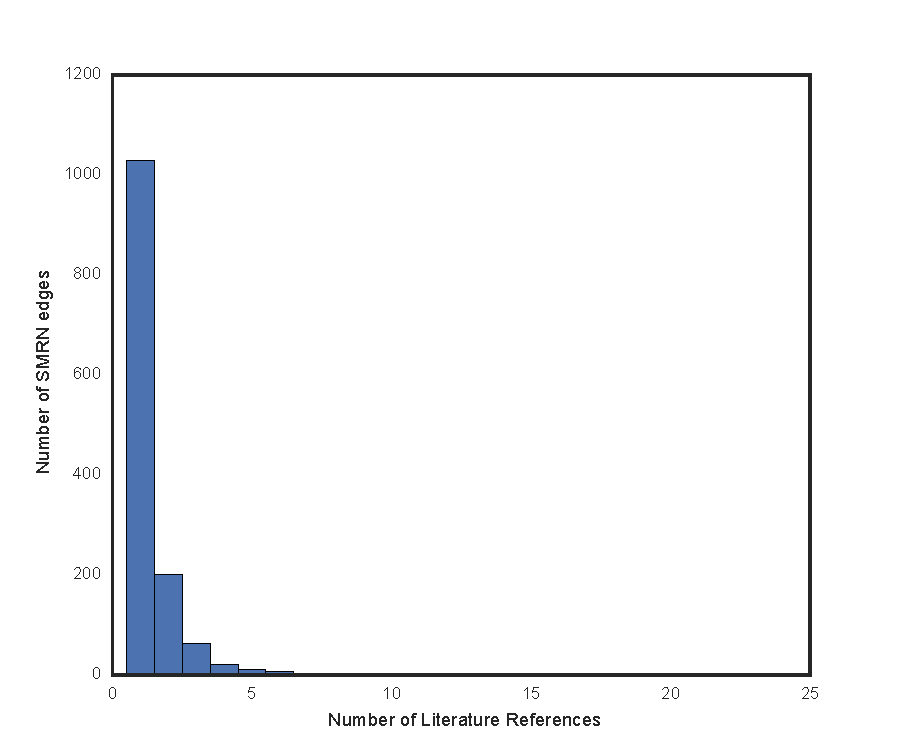
\includegraphics[width=\textwidth]{../manuscript/figS11.pdf}
	\caption{High confidence edges from literature}
\end{figure}

\end{document}
